\documentclass{amsart}
\usepackage{}
\usepackage{tikz}
\usetikzlibrary{arrows.meta}
\begin{document}
\title{Vehicle Priority Queues on Two-Lane Roads}
\author{David Prentiss}
\date{\today}
\maketitle
Consider a two-way, two-lane road segment connecting two at-grade, controlled
intersections. Suppose that in one direction, vehicles arrive at the upstream
end of their respective lane according to a Poisson process with mean arrival
rate $\lambda$. We will, for the moment, ignore the other lane.

Suppose also, that arriving vehicles are in one of two classes, $A$ or $B$.
Furthermore vehicles in each class arrive in equal proportion such that their
respective mean arrival rates are $\lambda_A=\lambda_B=\lambda/2$.
We leave the practical difference between the two classes deliberately abstract. However,
it may be useful to think of the two classes as being different intended turning motions.
For now, the only practical difference is that the downstream intersection
controls will admit only one class or the other in a single phase. Equivalently,
we could say that, during a single phase the intersection admits all and only
the vehicles of the same class that happen to be adjacent to each other at the
head of the queue. For example, if the sequence of vehicles starting from the head of the
queue had classes $\{A,B,B,A,A,A,B,B\}$, then the intersection would, in sequential
phases, admit one vehicle of type $A$, then two vehicles of type $B$, then three vehicles
of type $A$, and so on.

For the purposes of analysis, we make the following, additional simplifying
assumptions regarding vehicle dynamics.
First, time and space are discretized such that each vehicle takes the space of
one cell and can move, at most, one cell per time step.
The time then, for $n$ vehicles to enter the intersection is $T_n=n$ steps,
where $n$ is a random variable representing the number of vehicles admitted
through the intersection during a given phase.
Second, vehicles that enter the intersection are considered to have left the system.
And third, the time until the next phase is $T_n+T_p$, where $T_n = t(n)$ and $T_p$ is a random variable
representing the time necessary for the intersection to complete some other,
mutually exclusive activities such as another phase for vehicles in other,
un-modeled legs.
For now, we will say of $T_p$ only that it is i.i.d.\ as $T_n$.

We will take expected rate of departure, $\mu$ to be the expected value of
\begin{equation*}
  \frac{n}{T_n+T_p}.
\end{equation*}
Since $T_n=n$ steps/vehicle, then $\text{E}[n]=\text{E}[T_n]$ vehicles.
That is, the expected number of steps it takes the next group of vehicles to enter the
intersection is equal to the expected number of vehicles in that group. So we
have
\begin{equation*}
  \mu = \text{E}\left[\frac{n}{T_n+T_p}\right]
  =\text{E}\left[\frac{n}{n+n}\right] = \frac{1}{2}\text{ (vehicles/step)}.
\end{equation*}

Now suppose that we moved the stop bar back some number of cells $k$.

Then $\text{E}[T_n]=\text{E}[T_p]=\text{E}[n]+k$ and

\begin{equation*}
  \mu = \text{E}\left[\frac{n}{T_n+T_p}\right]
  = \text{E}\left[\frac{n}{2(n+k)}\right]
  = \frac{1}{2}\text{E}\left[\frac{n}{n+k}\right]
\end{equation*}

\end{document}

\section{Drafts}
\subsection{Equal length paths on a Manhattan grid}
\begin{figure}
  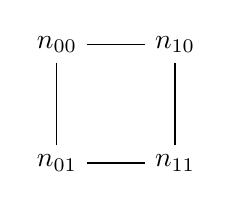
\begin{tikzpicture}[node distance={1.5cm}]
    \node (00) {$n_{00}$};
    \node (10) [right of=00] {$n_{10}$};
    \node (01) [below of=00] {$n_{01}$};
    \node (11) [right of=01] {$n_{11}$};

    \draw (00) edge (10);
    \draw (00) edge (01);
    \draw (10) edge (11);
    \draw (00) edge (10);
    \draw (01) edge (11);
  \end{tikzpicture}
\end{figure}
